\section{Mechanism Decomposition}
\label{sec:mechanism}

\subsection{Four-Condition Control}

\begin{figure}[t]
  \centering
  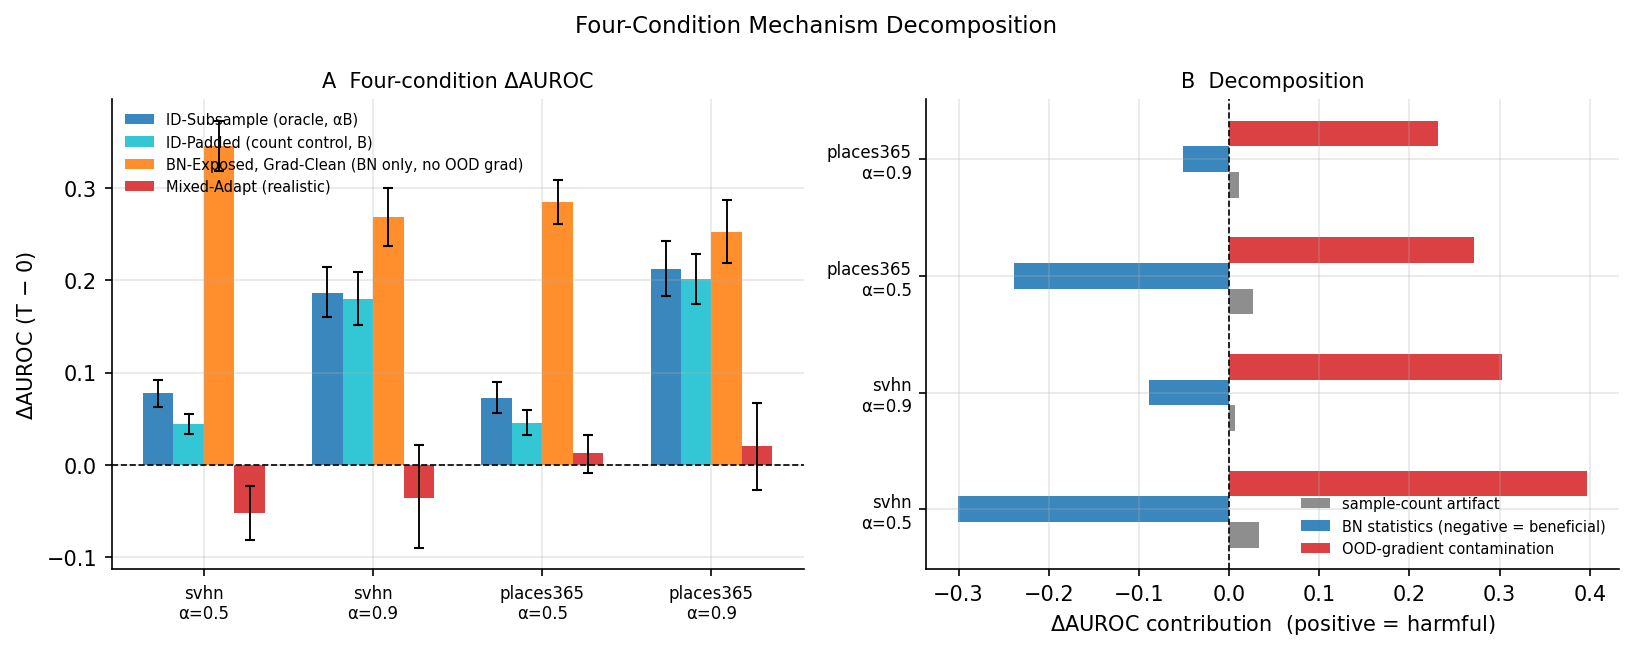
\includegraphics[width=\linewidth]{figures/fig4_decomposition.png}
  \caption{%
    \textbf{OOD gradient contamination, not BatchNorm statistics, is the dominant factor driving the paired gap.}
    \emph{Left (Panel A)}: Mean $\DeltaA$ for all four conditions across experimental cells.
    $\ml$ (BN sees OOD, gradient excludes OOD) dramatically outperforms the oracle $\idonly$ in every cell.
    $\mixed$ (full contamination) is the worst condition.
    \emph{Right (Panel B)}: Additive decomposition (Eq.~\ref{eq:decomp}).
    The BN component (blue, extending \emph{left}) is consistently negative---BN exposure to OOD helps.
    The gradient component (red, extending \emph{right}) is dominant and consistently positive.
  }
  \label{fig:decomposition}
\end{figure}

Table~\ref{tab:decomp} summarizes results from the four-condition control.
The most striking finding is that $\ml$ \emph{outperforms the oracle} $\idonly$ in every cell.
For SVHN $\alpha = 0.5$ under gaussian noise: $\DeltaA(\ml) = +0.345$ vs.\ $\DeltaA(\idonly) = +0.044$ ($4.4\times$ better).
BatchNorm computing joint statistics over heterogeneous ID and OOD images---instead of ID-only---creates contrast that the ID-restricted entropy loss exploits.

\begin{table}[t]
\centering\small
\caption{%
  Four-condition decomposition results (TENT, $n{=}30$, severity 5).
  All conditions use the same drawn batches.
  Decomposition percentages are relative to the total gap $(\idsub - \mixed)$.
}
\label{tab:decomp}
\begin{tabular}{llcccc r@{\,}r@{\,}r}
\toprule
OOD & $\alpha$ & $\idsub$ & $\idfull$ & $\ml$ & $\mixed$ & \multicolumn{3}{c}{Decomposition} \\
    &          &          &           &       &          & sample & BN & grad \\
\midrule
\multicolumn{9}{l}{\textit{gaussian noise}} \\
SVHN & 0.5 & $+0.078$ & $+0.044$ & $+0.345$ & $-0.052$ & $+25\%$ & $-232\%$ & $+306\%$ \\
SVHN & 0.9 & $+0.186$ & $+0.179$ & $+0.268$ & $-0.035$ & $+3\%$  & $-40\%$  & $+137\%$ \\
Places365 & 0.5 & $+0.072$ & $+0.046$ & $+0.285$ & $+0.012$ & $+45\%$ & $-400\%$ & $+456\%$ \\
Places365 & 0.9 & $+0.212$ & $+0.201$ & $+0.252$ & $+0.021$ & $+6\%$  & $-27\%$  & $+121\%$ \\
\midrule
\multicolumn{9}{l}{\textit{fog (replication)}} \\
SVHN & 0.5 & $+0.032$ & $+0.017$ & $+0.129$ & $-0.090$ & $+12\%$ & $-23\%$ & $+180\%$ \\
SVHN & 0.9 & $+0.087$ & $+0.083$ & $+0.114$ & $-0.050$ & $+3\%$  & $-92\%$ & $+120\%$ \\
\bottomrule
\end{tabular}
\end{table}

The BN contamination component $(\idfull - \ml)$ is \emph{negative} across all 6 cells, ranging from $-23\%$ to $-400\%$ of the total gap.
The gradient contamination component $(\ml - \mixed)$ is the dominant positive term, ranging from $+120\%$ to $+456\%$.
The sample-count artifact $(\idsub - \idfull)$ is small ($+3$--$+45\%$), confirming that batch-size differences do not explain the gap.

These findings overturn the prior hypothesis that shared BatchNorm statistics are the primary contamination mechanism.
The dominant mechanistic factor is direct OOD gradient contamination: when OOD samples appear in the entropy minimization objective, the model is explicitly optimized to produce confident predictions on OOD inputs, collapsing the ID/OOD score gap.

\subsection{Role of BatchNorm as a Gradient Amplifier}

\paragraph{BN vs. InstanceNorm ablation.}
Replacing BatchNorm with InstanceNorm (per-sample statistics) reduces the paired gap by 88.9\% ($p = 2.3 \times 10^{-9}$).
However, id-only $\DeltaA$ also drops by 86\%---InstanceNorm computes noisier statistics than batch statistics, weakening adaptation.
The contamination penalty as a fraction of adaptation gain is nearly identical: $1.67$ for BN-TENT vs.\ $1.36$ for IN-TENT.
The gap reduction reflects weaker adaptation overall, not a BN-statistics-specific pathway.

\paragraph{ViT-S/16 backbone.}
A ViT-S/16 \citep{vit} fine-tuned on CIFAR-10 (98.80\% test accuracy, LayerNorm throughout) shows a paired gap of $+0.013$ ($p = 2.6 \times 10^{-10}$, SVHN, $\alpha=0.5$, gaussian noise).
This matches the ResNet-18/InstanceNorm residual gap of $+0.014$.
Both architectures lack shared batch statistics; their matched residuals confirm that the gradient contamination pathway is a real, independent signal.
The $10\times$ difference between ResNet-18/BN (+0.130) and ViT (+0.013) reflects BN's stronger adaptation signal in both directions, not a BN-statistics contamination pathway.

\subsection{Why Partial Fixes Fail}

\paragraph{Fix A: confidence-weighted entropy.}
Down-weighting low-MSP (high-uncertainty) samples in the entropy loss does not reduce the paired gap ($p > 0.35$ at all $\alpha$).
Samples with moderate MSP---many of which are OOD---still contribute non-negligible gradient weight.
Partial gradient filtering is insufficient: the score gap collapses even with reduced OOD gradient.

\paragraph{Fix C: entropy threshold filtering.}
Removing the top-$\tau$ fraction of highest-entropy samples reduces the gap by $\sim 50\%$ for DTD at $\alpha = 0.5$ with $\tau \ge 0.3$, but fails for SVHN and for both OODs at $\alpha = 0.9$.
This is consistent with the gradient contamination mechanism: thresholding removes the most uncertain OOD samples but passes moderate-entropy OOD samples, leaving residual contamination.
The $\ml$ condition, which applies complete gradient exclusion while retaining BN exposure, provides a theoretical upper bound: it dramatically outperforms all partial fixes.
